%
% File naaclhlt2016.tex
% pdflatex paper.tex
% bibtex paper.aux
%
\documentclass[11pt,a4paper]{article}
\usepackage[hyperref]{acl2017}
\usepackage{times}
\usepackage{latexsym}
\usepackage{url}

%\usepackage{naaclhlt2016}
%\usepackage{times}
%\usepackage{latexsym}
\usepackage{bbm}
\usepackage{amsmath}
\usepackage[linesnumbered,ruled]{algorithm2e}
\usepackage{pbox}

\aclfinalcopy % Uncomment this line for the final submission

%\def\naaclpaperid{***} %  Enter the naacl Paper ID here

% To expand the titlebox for more authors, uncomment
% below and set accordingly.
% \addtolength\titlebox{.5in}    

\newcommand\BibTeX{B{\sc ib}\TeX}
\title{Deep Reinforcement Learning with Hierarchical Recurrent Encoder-Decoder for Conversation}
% Author information can be set in various styles:
% For several authors from the same institution:
% \author{Author 1 \and ... \and Author n \\
%         Address line \\ ... \\ Address line}
% if the names do not fit well on one line use
%         Author 1 \\ {\bf Author 2} \\ ... \\ {\bf Author n} \\
% For authors from different institutions:
% \author{Author 1 \\ Address line \\  ... \\ Address line
%         \And  ... \And
%         Author n \\ Address line \\ ... \\ Address line}
% To start a seperate ``row'' of authors use \AND, as in 
% \author{Author 1 \\ Address line \\  ... \\ Address line
%         \AND
%         Author 2 \\ Address line \\ ... \\ Address line \And
%         Author 3 \\ Address line \\ ... \\ Address line}
% If the title and author information does not fit in the area allocated,
% place \setlength\titlebox{<new height>} right after
% at the top, where <new height> can be something larger than 2.25in

\author{Heejing Jeong \and Xiao Ling\\
  {\tt [heejinj, lingxiao]@seas.upenn.edu}}
\date{}
\begin{document}
\maketitle

\begin{abstract}

This paper investigates the efficacy of combining deep reinforcement learning with a hierarchical recurrent encoder decoder for conversational dialogue systems. 

\end{abstract}

In recent years, numerous neural network based methods have been introduced for automatic dialog generation. Sutskever et al. presented a sequence to sequence learning model with deep neural networks (SEQ2SEQ) consisting of two multi-layered Long Short-Term Memory (LSTM) and showed that it outperformed a standard SMT-based system on an English to French translation task \cite{Sutskever}. Vinyals et al. applied this sequence to sequence framework to conversational modeling and their model predicted the next sentence given the previous sentence \cite{Vinyals}. Unlike other models that had been used widely, this model achieved better performance requiring much fewer hand-crafted rules. \\
However, since the SEQ2SEQ model was originally proposed for machine translation tasks, it does not capture previous conversations when it is applied to a conversation task. Being able to address previously mentioned topics or information is essential in conversation. In order to solve this issue, Serban et al. extended the hierarchical recurrent encoder-decoder (HRED), proposed by Sordoni et al. \cite{Sordoni}, to the dialog domain \cite{Serban}. Although they used only triple utterances for implementation, they were able to show their proposed model outperformed both $n$-gram based models and baseline neural network models. Another issue of the SEQ2SEQ model is that it tends to be short-sighted since the model does not consider its future outcomes. Addressing this issue, Li et al. proposed a novel approach for a dialog generation task combining a policy gradient optimization method and the SEQ2SEQ model (DRL-SEQ2SEQ) \cite{Li}. The policy gradient optimization method is one of policy-based methods in Reinforcement Learning (RL), and it updates its policy parameters in order to maximize a learner's expected discounted future total reward. Thus, we can expect the model would generate an outcome more likely to continue the current conversation. \\
While the HRED model does not consider its future outcomes, the DRL-SEQ2SEQ model cannot address its conversation history other than a few immediate previous utterances. In this project, we studied the HRED model for dialog generation in open domain \cite{Serban} and DRL-SEQ2SEQ. We initially aimed to replace SEQ2SEQ model in DRL-SEQ2SEQ with HRED in order to utilize the advantage of each model. However, due to the time constraint, we were not able to combine both models but tried implementing them on OpenSubtitle Dataset. 

In this section explain the hiearchical recurrent neural net (HRED) model proposed by \cite{Serban} and \cite{Sordoni}, the problem they posed and how HRED solves these problems. In the original paper by \cite{Sordoni}, HRED was proposed as a model that could generate context-senstitive queries, then \cite{Serban} adapted it to train an end-to-end history-aware conversation model.

\subsection{Recurrent Neural Net}

Now we wish to review recurrent neural net (RNN) in some detail. We denote a dialogue as a sequence of $M$ utterances $U_m$: $D = \{U_1, \ldots, U_M\}$ between two speakers, each utterance contains $N_m$ tokens: $U_m = \{w_{m,1},\ldots,w_{m,N_m}\}$. $\cite{Serban}$ allowed the random variable $w_{m,n}$ to range over the vocabular and ``speech acts", although in our case we only considered words. Next they defined a distribution $P$ with parameter $\theta$ over the set of all possible dialogues of any length, and factorized $P$ by:
    \begin{align*}
        P_{\theta}(U_1, \ldots, U_M) &= \prod_{m=1}^M P_{\theta}(U_m | U_{<m}) \\
                                     &= \prod_{m=1}^M \prod_{n=1}^{N_m} P_{\theta} (w_{m,n}|w_{m,<n}, U_{<m}),
    \end{align*}

where $U_{<m} = \{U_1, \ldots, U_{m-1}\}$. In other words, the conditional probability of the current word is only a function of previous words in the utterance and previous utterances. Next, \cite{Serban} represents $P_{\theta}$ with:
    \begin{align*}
        P_{\theta} (w_{n+1} = v | w_{\leq n}) = \frac{\exp(g(h_n,v))}{\sum_{v'} \exp(g(h_n, v'))},
    \end{align*}

where $h_n \in \mathbbm{R}^{d_h}$ is a hidden state computed by a recurrent neural net:

    \begin{align*}
        &h_n = tanh (H h_{n-1} + I_{w_n}) \\
        &g(h_n, v) = O^{T}_{w_n} h_n,
    \end{align*}

where $I \in \mathbbm{R}^{d_h \times |V|}$ is the input word embeding. Again note that the hidden state is only a function of the past. 

\subsection{Hierarchical Recurrent Neural Net}

HRED augments the basic RNN model by explicitly learning a transition function over the hidden dynamic of the conversation or  ``session". Serban and Sordoni learned this transition function using a session level RNN. Specifcially, this RNN predicts the next utterance by:
    \begin{align*}
        P(U_m|U_{<m}) &= \prod_{n=1}^{N_m} P(w_n | w_{<n-1}, U_{m-1}) \\
                      &= \frac{\exp(o_{v}^T w(d_{m,n-1}, w_{{m,n-1}}))}{\sum_{k} \exp(o_{k}^Tw(d_{m,n-1}, w_{m,n-1}))},
    \end{align*}

where $w(d_{m,n-1}, w_{m,n-1}) = H_o d_{m,n-1} + E_o w_{m,n-1} + b_o,$ so that the next utterance is a function of all pervious utterances. In summary, in HRED each utterance is a function of the previous utterance, and each word in the utterance is a function of all previous words in the utterance. A session level RNN learns the transition between utterances vector, and sentence level RNN learns the transition between words. 

\subsection{Learning}

HRED is trained end-to-end by maximizing the log-likelihood of the whole session $S$:

    \begin{align*}
        Loss(S) &= \sum_{m=1}^M log P(U_m|U_{<m}) \\
                &= \sum_{m=1}^M \sum_{n=1}^{N_m} log P(w_{m,n} | w_{m,<n}, U_{<m}).
    \end{align*}

We train the model by dividing the data set into sessions with four utterances each, the vocabulary size was set to be 50,005, and the maximum sentence length was 50 tokens.





































In the RL framework, there is a learner in a certain state $s$ and the learner executes an action $a$ to an environment based on her action policy $\pi^{(a)}$. Then, the environment gives a feedback in a form of a reward, $r$, and the learner updates her optimal policy $\pi^*$ in order to maximize her expected discounted future total reward: 
\[
	\mathbf{E}[r_t + \gamma r_{t+1} + \cdots + \gamma^{T-t}r_T | s_t, \pi^* ]
\]
where $T$ is time horizon and $\gamma$ is a discount factor which controls the relative importance of the immediate reward for the learner. If $\pi^{(a)}$ differs from $\pi^*$, the learning method is categorized to \textit{off-policy}, and if $\pi^{(a)} = \pi^*$, the method is \textit{on-policy}. In order to apply RL to a certain learning task, we need to define an appropriate learning system first. In this project, we followed the learning system defined in the DRL-SEQ2SEQ paper \cite{Li}. 

\subsection{Learning System for Dialog Generation}
The learning system consists of two agents where they take turns talking with each other. Unlike the notations in the paper, we will use $u_i$ as a notation for the $i$-th utterance of a conversation regardless which agent spoke it in order to make sure that the learning model is trained with both agents. \\
A state is defined by the previous two dialog turns, $s_t = [u_{t-1}, u_t]$. Specifically, the concatenated vector of the two utterance vectors is used as an input of the SEQ2SEQ encoder. An action $a$ is defined as a dialog utterance to generate. The action space, $\mathcal{A}$, is considered as an infinite space, but we constrained the maximum length of the generated utterance, $L$, and the number of available vocabularies, $|V|$ ($V$ is a set of available vocabulary). Therefore, $|\mathcal{A}|=L\times |V|$ in our model. The RL policy, $p_{RL}$, uses the form of a SEQ2SEQ encoder-decoder defined by its parameters. 

\subsection{Reward}
Li et al. defined three reward functions and used the weighted sum of the rewards as a total reward \cite{Li}. The first reward function measures the ease of answering a generated turn (or action) using the log likelihood of responding to that action with a dull response. They defined dull responses with 8 turns including "I don't know what you are talking about", "I have no idea", etc. The function is:
\begin{equation}
	r_{1,t} = -\frac{1}{N_{\mathcal{D}}} \sum_{d\in \mathcal{D}} \frac{1}{|d|} \log p_{seq2seq}(d|a_t)
\end{equation} 
where $\mathcal{D}$ is a set of dull responses and $p_{seq2seq}$ is a probability distribution with parameters learned by SEQ2SEQ. $p_{seq2seq}$ is different from $p_{RL}$. \\
The second reward function penalizes semantic similarity between consecutive turns from the same agent. They used cosine similarity to measure:
\begin{equation}
	r_{2,t} = -\log \cos (h_{u_{t-1}}, h_{a_t}) = -\log \cos \frac{h_{u_{t-1}}\cdot h_{a_t}}{||h_{u_{t-1}}||_2 ||h_{a_t}||_2} \label{eq:reward2}
\end{equation}
where $h_{u_{t}}$ is an SEQ2SEQ encoder output with the input $u_t$. \\
The last reward function addresses semantic coherence considering mutual information:
\begin{equation}
r_{3,t} = \frac{1}{|a_t|} \log p_{seq2seq} (a_t|u_{t-1},u_t) + \frac{1}{|u_t|} \log p_{seq2seq}^{backward}(u_t|a_t) \label{eq:reward3}
\end{equation}
where $ p_{seq2seq}^{backward}$ the probability distribution with parameters learned by SEQ2SEQ where sources and targets are swapped. Therefore, this backward SEQ2SEQ model has to be separately trained before using the RL rewards. 

\subsection{Model}
\begin{figure}[b!]
    \centering
    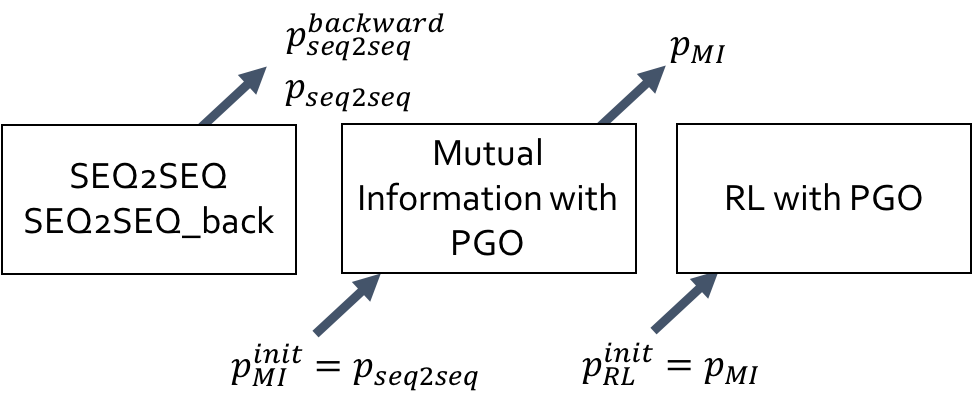
\includegraphics[width=0.4\textwidth]{three_steps.png} 
    \label{fig:three_steps}
    \caption{\small Training Procedure of the proposed Reinforcement Learning Model}
 \end{figure}
Any RL method falls into one of policy-based, value-based, or actor-critic RL areas. Among policy-based RL methods, a policy gradient optimization (PGO) using REINFORCE algorithm \cite{Williams} has been widely used. Li et al. also used the REINFORCE algorithm for learning the RL model. The training procedure of the RL model is divided into three steps as shown in the Fig.\ref{fig:three_steps}. First, we train a SEQ2SEQ model and a SEQ2SEQ backward model. Next, we train a mutual information model learned by PGO maximizing the semantic coherence (Eq.\ref{eq:reward3}). The policy parameters of the model are initialized by the parameters of the pre-trained SEQ2SEQ model, and its objective function is:
\begin{equation}
	J(\theta)= 	\mathbf{E} [m(\hat{a},[u_{t-1},u_t])] \label{eq:obj_func}
\end{equation}
where $m(\hat{a},[u_{t-1},u_t])$ is equal to $r_{3,t}$ in the Eq.\ref{eq:reward3}. The gradient is estimated using the likelihood ratio trick in PGO:
\begin{equation}
	\nabla J(\theta) = m(\hat{a},[u_{t-1},u_t]) \nabla \log p_{RL}(\hat{a},[u_{t-1},u_t]) \label{eq:gradient}
\end{equation}

Then, we update the parameters in the encoder-decoder model using stochastic gradient ascent. In addition to the standard PGO method, Li et al. adopted a curriculum learning strategy proposed by Ranzato et al. \cite{Ranzato} and a baseline strategy. The baseline strategy is common in implementing PGO method since PGO tends to have high variance, and the strategy helps to reduce the variance.

\vskip 1\baselineskip

\bibliography{paper}
\bibliographystyle{acl_natbib}

\end{document}



